\chapter{Fejlesztői dokumentáció}
\label{ch:impl}

Az alkalmazás a könnyű megközelíthetőség miatt web alapúan kerül megvalósításra. Ennek számos előnye van. Az alkalmazás nem igényel telepítést, bármilyen számítógépről, bármikor elérhető. A már ismert webes technológiákat alkalmazhatjuk. És Progresszív Web Alkalmazás (PWA \cite{PWA}) lévén az első megnyitást leszámítva aktív internetelérés sem kell a használatához.

\section{Megoldási terv}

Az alkalmazás fő eleme a projekt amit Lore-nak nevezünk, ennek an egy aznosítója mivel dokumentum szintű objektumról van szó, egy neve és ebben tároljuk a világ adatait melyek annak mérete és neve. Valamint ehhez a dokumentumhoz tartozik a világ textúrája is.

Egy projecthez tartoznak még szereplők amik szintén dokumentum szintű objektumok, saját kollekcióval. Ebben tároljuk a szereplő állapotait egy AVL fában \cite{AVL} amiben a kulcs az idő, ezzel biztosítva, hogy minden esemény időben sorban legyen, és gyorsan elérhetőek legyenek. Szükség lesz ehhez a fához néhány segédeljárásra, szerencsére ezen TypeScript implementációja az AVL fának az enyém így ezeket könnyedén hozzáadhatom. A fő motiváló ereje ennek a segédcsomagnak a létrehozására épp az volt, hogy az alapvető implementáció mellé egy gazdag API-t biztosítsak.

Egy állapotdelta csak az előző állapotdeltákhoz viszonyított különbséget tartja nyilván, kivéve a pozíciót, ami minden esetben kötelező. Ezeket a deltákat a szereplők és a jelenlegi idő csöveinek összevezetésével egy aggregátoreljárás értékeli ki. Erre feliratkozva bármi azonnal hozzáférhet a legfrissebb adatokhoz ami csak egy helyen, egyszer van emiatt kiszámolva.

\subsection{Az adatmodell}
\begin{plantuml}
@startuml
skinparam monochrome true

note left of Lore: Tartozhat minden példányhoz egy\nRxDocument 'texture' azonosítóval

interface Lore {
	id: string
	name: string
	planet: Planet
}

interface Planet {
	name: string
	radius: number
}

interface Actor {
	id: string
	loreId: string
	states: Tree
}

note left of Tree: Nem perzisztálható de szérializálható
class Tree {
	root: Node
}

class Node {
	key: number
	value: ActorDelta
}

note left of ActorDelta: Egy AVL\nfában helyezkednek el
interface ActorDelta {
	position: Vec3
	name?: string
	maxSpeed?: number
	color?: string
	properties?: Array<Property>
}

interface Vec3 {
	x: number
	y: number
	z: number
}

interface Property {
	key: string
	value: string
}

Lore -- Planet
Lore --o Actor
Actor -- Tree
Tree --* Node
Node -- ActorDelta

ActorDelta --* Property
ActorDelta -- Vec3

@enduml
\caption{Az adatmodell}
\label{fig:data-model}
\end{plantuml}

\pagebreak

Az alkalmazás induláskor az adatbázis modelljeit tároló kollekiókat inicializáljuk.

\begin{plantuml}
	@startuml
	hide empty description
	skinparam monochrome true

	state DatabaseBootstrap {
		[*] --> InitializeCollections
		InitializeCollections : Lore
		InitializeCollections : Actor
		InitializeCollections : ActorDelta
		InitializeCollections --> InitializeExample
		InitializeExample --> [*]
		note right of InitializeCollections : Ez a folyamat csak akkor\nhozza létre a kollekciókat\nha szükség van rá
		note right of InitializeExample : Az alap project létrehozása
	}

	DatabaseBootstrap --> DatabaseBootstrap : On Fail

	@enduml
\end{plantuml}

\subsection{Reaktív elemek}

Az alkalmazás jelentős részében reaktív komponenseket használunk amik alapjául az RxJS \cite{RxJS} csomag szolgál. Ez azt jelenti, hogy klasszikus adattagok helyett, adatforrásokat, megfigyelhető objektumokat (Lásd Megfigyelő programtervezési minta \cite{ObserverPattern}), függvényhívások helyett pedig mellékhatásokat használunk.

Ez a minta lehetőséget ad arra, hogy bármilyen nézet a böngészőben ami felhasznál valamilyen adatot, azonnal frissüljön mikor a forrása megváltozik.

\begin{figure}[h!]
	\centering
	\begin{plantuml}
		@startuml
		skinparam monochrome true
		hide empty description
		[*] -> Observable : Új adat kerül a megfigyelhető objektumba
		Observable --> Pipes
		Pipes : A csövek formában és időben is \nmegváltoztathatják a bennük átfolyó adatot
		Pipes --> SideEffects : A transzformáció közben mellékhatásokat is definiálhatunk
		Pipes --> ObserversA
		Pipes --> ObserversB
		Pipes --> ObserversC : Majd pedig megérkeznek minden feliratkozóhoz

		SideEffects  --> [*]
		ObserversA --> [*]
		ObserversB --> [*]
		ObserversC --> [*] : És kifejtik hatásukat
		@enduml
	\end{plantuml}
	\caption{Adatfolyam a megfigyelő modellben}
	\label{fig:observer-pattern}
\end{figure}

Kétfajta adatot különböztetünk meg, perzisztens és temporális. Perzisztens adatnak minősül minden ami egy projekthez tartozik. Temporális meg az amiket az előbbi manipulálásakor használunk fel. Például projekthez tartozó adat az, hogy egy szereplőnk egy adott időpillanatban hol tartózkodik, de az nem, hogy a kurzor épp ezen az időpillanaton áll.

A perzisztens a böngészők beépített noSQL adatbázisában, az IndexedDB-ben kerülnek perzisztálásra, dokumentumok formájában. Az adatbázis elérésehez, és ezzel az alkalmazás reaktív modelljének alapkövének RxDB-t \cite{RxDB} használunk.

Ez a csomag lehetővé teszi, hogy adatok beszúrásakor/módosításakor/törlésekor ezek a folyamatok igéretekként (Lásd Promise \cite{Promise}) jelenjenek meg melyek teljesüléséről értesítést kapunk. Ezzel lehetővé téve olyan featureöket mint, hogy jelezni a felhasználónak, hogy egy adott elem adatainak forrása éppen mentés alatt áll, és a szerkesztését letiltani. A legfőbb előnye viszont az, hogy bármilyen adatbázis kollekciót, lekérdezést megfigyelhetünk. És amint változás történik az adatbázisban, ezek a megfigyelhető Query-k újra jeleznek, frissítve minden mást ami rájuk épül.

A temporális adatokat viszont felesleges adatbázisban tárolni csak azért, hogy reaktív módon kezelhessük őket. Lehetőség van minden ilyen adatnak egy saját forrást (Subject) biztosítani. De mi van ha két adat függ egymástól? Csöveken keresztül futtassuk őket össze, válasszuk szét majd az így keletkező csöveket használjuk ezentúl? Mi van ha erre a változtatásra később kerül sor? Mi van ha valamit elfelejtünk átállítani, hogy a direkt-forrás helyett a transzformált csövet használják? Ezek a problémák és még sok más megoldására jön képbe az NgRX \cite{NgRx} csomag és a Redux (\cite{Redux}) architektúra amit implementál.

\begin{figure}[h!]
	\centering
	\begin{plantuml}
		@startuml
		skinparam monochrome true
		hide empty description
		[*] -d-> View : Felhasználói interakció
		View -d-> Dispatcher : Akció
		Dispatcher -l-> Effects : Akció
		Effects -r-> Dispatcher : Akció
		Effects -l-> [*] : Mellékhatás

		Dispatcher --> Reducer : Akció
		CurrentState -> Reducer : Az előző állapot
		Reducer --> Store : Új állapot készül
		Store -u-> View : Értesít

		@enduml
	\end{plantuml}
	\caption{A Redux architektúra}
	\label{fig:redux-architecture}
\end{figure}

A lényeg a globális, nem módosítható (Csak cserélhető) állapot, az úgynevezett "igazság egyetlen forrása" ("Single source of truth") és az egyirányú adatfolyam (Unidirectional data-flow). Ennek hála egy átlátható, eseményeiben könnyen megjósolható programot kapunk, cserébe viszont sok kódot igényel.
Ezt egy központi Store service-ből tudjuk elérni, a könnyebb interakció miatt pedig egy Facade\cite{Facade} Service-t húzunk elé.

\section{Alkalmazás Architektúra}

Egy Angular alkalmazás modulokra van bontva. Minden modul saját Injection Scope-al rendelkezik, a felhasznált Service-ek pedig egyediek Injection Scope-onként. Mivel ez az alkalmazás csupán egy funkciót lát el megelégedhetnénk egy modullal is, de jobb felhasználói élményt érhetünk el ha az első töltést felgyorsítjuk azzal, hogy az applikációnk első töltési pontját kiürítjük, a tényleges applikációt pedig a gyökér routing pont mögé tesszük. Ez lusta módon \cite{LazyLoad} fogja betölteni a tényleges tartalommal rendelkező modult, nem blokkolva az alap modul tartalmának festését a DOM-ba. Az alap modul így taralmazhat egy egyszerű töltési animációt amit csak addig jelenítünk meg amíg a router tölti az almodult.

\begin{figure}[h!]
	\centering
	\begin{plantuml}
		@startuml
		skinparam monochrome true

		[-> AppModule: Applikáció indításakor
		activate AppModule
		AppModule -> AppModule : Első festés, LoreModule Lazy töltése

		activate  AppModule
		AppModule -> LoreModule
		deactivate AppModule

		activate LoreModule

		LoreModule ->]
		LoreModule <-]


		AppModule <- LoreModule: Kilépés
		deactivate LoreModule

		[<- AppModule: Kilépés
		deactivate AppModule

		@enduml


	\end{plantuml}
	\caption{Lusta betöltés}
	\label{fig:lazy-loading}
\end{figure}


\subsection{Komponensek}

Nézeteinket komponensekben definiáljuk, ezek az adataikat pedig kizárólag a StoreFacade-on keresztül kapják. Egyedül az Engine és a 3D színtér az ami közvetlen az adatbázissal kommunikál.

\begin{figure}[h!]
	\centering
	\begin{plantuml}
		@startuml
		skinparam monochrome true

		database IndexedDB {
			[LoreCollection]
			[ActorCollection]
		}

		database Store {
			[State]
		}

		IndexedDB -[hidden]--> LoreModule
		Store -[hidden]--> LoreModule

		IndexedDB .> (RxDB)


		package LoreModule {
			Store .> (StoreFacade)
			(RxDB) ..> (DatabaseService)
			(DatabaseService) .[hidden].> [Lore]
			(DatabaseService) <.> Engine
			Store <.. (DatabaseService)
			(StoreFacade) .> [Lore]
			(StoreFacade) .> Components
			(StoreFacade) .> Engine
			[Lore] <- Components
			node Components {

				node Control {
					[LightControl]
					[SceneControl]
					[PlayControl] --> [SpeedControl]
				}


				node Timeline {
					[Block] --> [Timeline]
					[Cursor] --> [Timeline]
				}
			}

			[Lore] <- Engine

			Engine -[hidden]-> Components

			node Engine {
				(EngineService)
				[EngineComponent]
			}


		}


		@enduml
	\end{plantuml}
	\caption{Főbb Komponensek és relációik}
	\label{fig:services-and-components}
\end{figure}


\begin{figure}[h!]
	\centering
	\begin{plantuml}
		@startuml
		skinparam monochrome true
		== Initialization ==
		[-> Database : Database Initialized
		Database --> LoreState: Load Lores
		activate LoreState
		LoreState -> LoreState: Shim each entry
		LoreState ->]: loadLoresSuccess
		deactivate LoreState
		== Loading Lores ==
		note left of LoreState : updateInitialSelectedLore
		[-> LoreState : loadLoresSuccess
		activate LoreState
		LoreState -> LoreState: Select the first one
		LoreState ->] : changeSelectedLore
		deactivate LoreState
		== On Create Lore ==
		Database --> LoreState: createLoreSuccess
		LoreState ->]: changeSelectedLore
		== On Change Selected ==
		[-> LoreState: changeSelectedLore
		LoreState ->]: changeSelectedLoreSuccess
		== Change Selected ==
		[-> ActorState: changeSelectedLoreSuccess
		activate ActorState
		Database --> ActorState: connection
		ActorState -> ActorState: Loading everything into state
		ActorState ->]: loadActorsSuccess
		deactivate ActorState
		== On Load Actors ==
		[-> ActorState: loadActorsSuccess
		activate ActorState
		ActorState -> ActorState: Deserilization of deltas
		deactivate ActorState
		@enduml
	\end{plantuml}
	\caption{Bootstrap folyamatok}
	\label{fig:global-state-bootstrap}
\end{figure}


\subsection{Timeline}

Az idő az egész alkalmazásban epoch \cite{Epoch} formában van jelen, egy egyszerű számként, az egység a másodperc. Így könnyű egyszerű arithmetikai műveleteket végezni rajta.

Az idővonalat két időpont határoz meg, az eleje és a vége. A nézet szélességét figyelembe véve ezekből ki lehet számolni a vonalzó beosztásait. A beosztásokat napokban mérjük, az albeosztásokat pedig órában.

\subsubsection{Megjelenítés}

A beosztások mennyiségét és pozícióit ki kell számolnunk. Előbbit úgy kapjuk meg ha vesszük a megjelenített időablak hosszát és leosztjuk egy nappal ($86400s$). Az egészrésze lesz a kiférő beosztások száma. Viszont az albeosztások megjelenítésére is figyelnünk kell. Ezek fixen a tőle balra álló nagy beosztástól fognak elhelyezkedni. Ahhoz, hogy az idővonal legelején is lehessenek albeosztások -- az első látszódó beosztás előtt -- el kell tolnunk balra egy egységgel az idővonalat, és a végére még kettőt hozzáadni. Egy beosztás hosszát így kaphatjuk meg:

\begin{tabular}{@{}ll@{}}
	\textbf{Jel} & \textbf{Leírás} \\
	$a$ & Időablak kezdete \\
	$b$ & Időablak vége \\
	$d$ & A beosztás hossza ($86400$) \\
	$w$ & A komponens szélessége pixelben \\
	$d'$ & A beosztás szélessége pixelben \\
\end{tabular}
$$d' = \frac{w}{(b - a) / d}$$

A beosztások pozícióinak kiszámolásához, ahelyett, hogy minden beosztás helyét egyenként kiszámolnánk, csupán az első helyét számoljuk ki, a többit pedig ahhoz mérten, fix távolságban eltoljuk. Ezt azért tehetjük meg mert a beosztások egyenlő közönként vannak az idővonal egészén. Elég egyszer kiszámolni, hogy a $86400$ másodperc éppen mekkora távolságot jelent pixelben a képernyőn. Azután elég ennek a többszöröseit hozzáadni az első távolságához, minden egyes beosztásnál.

Az első távolság kiszámolásához viszont tudnunk kell, hogy melyik az a pont a kiválaszott időablakban ami egy napfordulót jelent:

$$ x \in \{[a, a+l] | x \% b = 0\} $$

Ehhez csak hozzá kell adni a beosztás hossza és a kezdeti érték maradékát a kezdeti értékhez miután kivontuk a beosztás hosszából:

$$x = a + (d - (a \% d))$$

Az albeosztásokat már tudjuk, hogy $24 - 1$ darab fog kelleni, kezdeti pozíciójuk meg nem számít, relatív a nagy beosztáshoz vannak elhelyezve. Csak azt kell kiszámolnunk, hogy az adott albeosztás másodpercben mennyit jelent ($0, 3600, 7200 \dots $) és pixelben mért távolsággá alakítani.


A két tartomány között lineárisan váltunk. A főbeosztások esetén a kezdeti tartomány az időablak, a céltartomány pedig a $[0, w]$ ahol $w$ a komponens szélessége. Az albeosztások esetén pedig $[0, 86400]$ ból váltunk $[0, d']$ be ahol $d'$ a beosztás hossza pixelben.

\begin{tabular}{@{}ll@{}}
	\textbf{Jel} & \textbf{Leírás} \\
	$x$ & A transzformálandó érték \\
	$a1$ & A forrás tartomány kezdete \\
	$a2$ & A forrás tartomány vége \\
	$b1$ & A cél tartomány kezdete \\
	$b2$ & A cél tartomány vége \\
\end{tabular}

$$ f(x) = b1 + ( x - a1 ) * ( b2 - b1 ) / ( a2 - a1 )$$

A beosztások mostmár helyesen helyezkedenek el minden időablak esetében.

\subsubsection{Manipulálás}

\paragraph{Folytonos manipuláláskor} mint például mikor pásztázunk az egerünkkel a kapott eseményben csak az eltolás mértékét kapjuk meg pixelben, ahhoz a pozícióhoz képest, ahol az elsolás kezdetekor az egér volt. A legtöbb ilyen esethez ezért definiálunk egy módszert amiben egy ilyen módon manipulálható adat mellé egy felülíró adattagot is definiálunk. Ez az adattag amikor nem történik esemény mindig \lstinline[columns=fixed]{undefined}.

Kiolvasni az adatpárost emiatt rövidzár kiértékeléssel egyszerű (\lstinline[columns=fixed]{override | original}). Fontos megjegyezni, hogy számok lévén, és mivel itt nem az adattag létezését vizsgáljuk hanem azt, hogy truthy e vagy sem, ha az \lstinline[columns=fixed]{override} értéke $0$ lenne, akkor ugyagyúgy az \lstinline[columns=fixed]{original} értékkel térne vissza a kifejezés. Mivel a $0$ az falsy. Így ezt csak akkor alkalmazzuk, ha tudjuk hogy ez az érték sosem lesz $0$. A másik megjegyzendő dolog, hogy miért nem egy osztályt definiálunk ennek a viselkedésnek a kezelésére. A válasz az, hogy ezek az adatok az állapot részét képezik, az állandó szérializálás és deszérializálás pedig túl sok extra komplexitást adna egy egyébként egyszerű feladathoz.

A folytonos manipuláció végén pedig az \lstinline[columns=fixed]{override} értékét beleírjuk az eredeti változóba majd kiürítjük.


A megjelenített időablakot kétféle módon manipulálhatjuk:

\begin{itemize}
	\item Eltolás (Translate)
	\item Merőleges affinitás (Scale)
\end{itemize}

\paragraph{Eltolásnál} csak egyenlő időmennyiséget vonunk ki vagy adunk hozzá az időablak mindkét végéhez

\paragraph{Affinitáshoz} pedig elég lenne ha nyújtásnál a kezdeti pontból kivonnánk, összenyomásnál pedig hozzáadnánk, a végpontból meg fordítva. Ezzel viszont mindig az időablak közepe lenne a sarkpontunk. A felhasználói élmény miatt ez a sarkpont mindig az egér pozíciója lesz. Szélsőséges esetekben, mikor az egész a komponens legelején helyezkedik el ez azt jeleti, hogy zoom-olásnál csak az időablak vége változik.

Ehhez a két vég módosítását súlyoznunk kell az egér pozíciója szerint. A pozíciót a böngésző belső ablakához relatív kapjuk meg, így a lineáris váltás kezdeti tartománya ${ta, ta + w}$ ahol $ta$ a timeline pozíciója horizontálisan, a céltartomány pedig $[0, 1]$. A kezeti pozíció súlya ez a szám lesz, a végéé pedig ehhez fordítottan arányos.

\subsubsection{A kurzor}

A kurzor egy időpontot jelöl. A színtérben, és a viewben minden aggregált adat ennek függvényében jelenik meg. Pozícióját hasonlóan az eddigikhez lineáris mappeléssel kapjuk meg. Manipulásakor pedig ugyanez történik visszafele.

\subsubsection{A blokkok}

Az idővonal sávjaiban a szereplő egy blokként jelenik meg. Egy blokknak -- hasonlóan az idővonalhoz -- van egy eleje és egy vége. Ezen belül pedig az események elemei helyezkednek el. A blokk eleje és vége mindig az első és az utolsó esemény ideje. Az események pozíciói a blokk elejének pozíciójához mérjük relatív.

Egy esemény idejének felülírásakor (Fogd-és-vidd ideje alatt) a gyakori változás miatt a fa-szerkezetet amiben az események vannak tárolva nem módosítjuk. Ehelyett egy felülírt esemény eseményt küldünk amiben leírjuk, hogy idő szerint melyik esemény hova került át. A színtér ezt az információt figyelembevéve módosítás közben is helyes adatokat tud kirajzolni.

\section{A színtér}

A 3D színtér komponensén két elem található: A canvas elem amire fest a Three.js és a buborékmenü ami a kijelölt szereplők felett helyezkedik el ha van ilyen. Erre a canvas elemre van felcsatolva az összes EventListener amivel interakcióba lehet lépni a színtérrel. Logikája annyiból áll, hogy ezeket az eseményekből kinyeri a hasznos információt, a pozíciót normalizálja a $[0-1]$ intervallumba, majd továbbítja az EngineService-nek ami aztán ezeket kezeli. Valamint megjelenítés után létrehozza a színtér modelljét és elindítja az animációs loopot.

\subsection{A színpad felépítése}

A színpad fő eleme a bolygó, egy fix $1$ sugarú gömb melyhez kapcsolódik egy másik, kisebb -- $0.98$ sugarú -- gömb ami a vízszintet reprezentálja. A gömb felszíne magas felbontású poligonok terén ($512×512$), hogy a displacement map \cite{Displacement} pontosabb eredeményt adjon.

Ekkora felbontásnál, az egy objektumon található rengeteg háromszög miatt a raycasting \cite{Raycast} rendkívül lassú a Three.js alap implementációjában. (Raycastingot akkor használunk amikor kiszámoljuk, hogy a színtér épp melyik objektumának melyik pontja felett áll az egér.) Szerencsére létezik gyorsabb eljárás. A Bounding Volume Hierarchy \cite{BVH} fa struktúrába helyezi az objektumok részeit elhelyezésük alapján, jelentősen lecsökkentve azokat a háromszögeket amiket a raycastingnak egyszerre meg kell vizsgálnia.

\begin{figure}[h!]
	\centering

	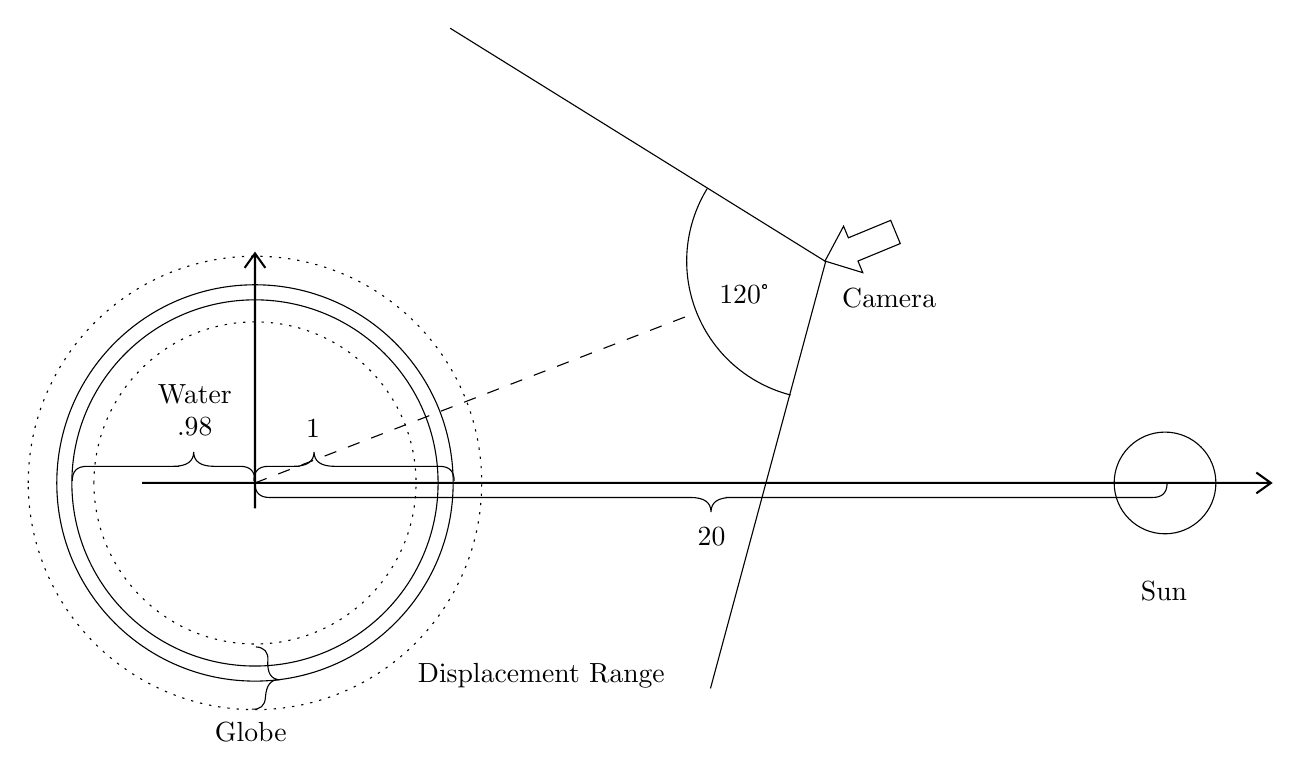
\begin{tikzpicture}[x=0.75pt,y=0.75pt,yscale=-1,xscale=1]
	%uncomment if require: \path (0,300); %set diagram left start at 0, and has height of 300

	%Shape: Circle [id:dp8728808526292304]
	\draw   (45.55,152) .. controls (45.55,99.27) and (88.3,56.52) .. (141.04,56.52) .. controls (193.77,56.52) and (236.52,99.27) .. (236.52,152) .. controls (236.52,204.73) and (193.77,247.48) .. (141.04,247.48) .. controls (88.3,247.48) and (45.55,204.73) .. (45.55,152) -- cycle ;
	%Shape: Circle [id:dp5674056113092418]
	\draw   (555,152) .. controls (555,138.47) and (565.97,127.5) .. (579.5,127.5) .. controls (593.03,127.5) and (604,138.47) .. (604,152) .. controls (604,165.53) and (593.03,176.5) .. (579.5,176.5) .. controls (565.97,176.5) and (555,165.53) .. (555,152) -- cycle ;
	%Shape: Axis 2D [id:dp667037457037013]
	\draw [line width=0.75]  (86.65,152) -- (630.5,152)(141.04,41.39) -- (141.04,164.29) (623.5,147) -- (630.5,152) -- (623.5,157) (136.04,48.39) -- (141.04,41.39) -- (146.04,48.39)  ;
	%Shape: Brace [id:dp5709274682232908]
	\draw   (141,152) .. controls (141,156.67) and (143.33,159) .. (148,159) -- (350.75,159) .. controls (357.42,159) and (360.75,161.33) .. (360.75,166) .. controls (360.75,161.33) and (364.08,159) .. (370.75,159)(367.75,159) -- (573.5,159) .. controls (578.17,159) and (580.5,156.67) .. (580.5,152) ;
	%Shape: Brace [id:dp38726825382608787]
	\draw   (237,151) .. controls (237,146.33) and (234.67,144) .. (230,144) -- (179.5,144) .. controls (172.83,144) and (169.5,141.67) .. (169.5,137) .. controls (169.5,141.67) and (166.17,144) .. (159.5,144)(162.5,144) -- (147.5,144) .. controls (142.83,144) and (140.5,146.33) .. (140.5,151) ;
	%Shape: Circle [id:dp559047975094662]
	\draw   (52.81,152) .. controls (52.81,103.28) and (92.31,63.78) .. (141.04,63.78) .. controls (189.76,63.78) and (229.26,103.28) .. (229.26,152) .. controls (229.26,200.72) and (189.76,240.22) .. (141.04,240.22) .. controls (92.31,240.22) and (52.81,200.72) .. (52.81,152) -- cycle ;
	%Shape: Brace [id:dp5585435570718464]
	\draw   (141,151) .. controls (141,146.33) and (138.67,144) .. (134,144) -- (121.5,144) .. controls (114.83,144) and (111.5,141.67) .. (111.5,137) .. controls (111.5,141.67) and (108.17,144) .. (101.5,144)(104.5,144) -- (60,144) .. controls (55.33,144) and (53,146.33) .. (53,151) ;
	%Left Arrow [id:dp007055379911458548]
	\draw   (415.67,45.1) -- (424.63,28.3) -- (426.94,33.9) -- (447.32,25.48) -- (451.94,36.67) -- (431.56,45.08) -- (433.87,50.68) -- cycle ;
	%Straight Lines [id:da28328227472011247]
	\draw  [dash pattern={on 4.5pt off 4.5pt}]  (141.04,152) -- (353.5,70) ;


	\draw   (235.08,-67.08) -- (416,45.34) -- (360.5,251) ;
	%Shape: Arc [id:dp11489271218380304]
	\draw  [draw opacity=0] (399.13,109.64) .. controls (379.34,104.55) and (362.14,90.46) .. (353.9,70.06) .. controls (345.66,49.66) and (348.24,27.59) .. (358.93,10.18) -- (415.67,45.1) -- cycle ; \draw   (399.13,109.64) .. controls (379.34,104.55) and (362.14,90.46) .. (353.9,70.06) .. controls (345.66,49.66) and (348.24,27.59) .. (358.93,10.18) ;
	%Shape: Circle [id:dp18625067716272725]
	\draw  [dash pattern={on 0.84pt off 2.51pt}] (31.79,152) .. controls (31.79,91.67) and (80.7,42.76) .. (141.04,42.76) .. controls (201.37,42.76) and (250.28,91.67) .. (250.28,152) .. controls (250.28,212.33) and (201.37,261.24) .. (141.04,261.24) .. controls (80.7,261.24) and (31.79,212.33) .. (31.79,152) -- cycle ;
	%Shape: Circle [id:dp21219909757761868]
	\draw  [dash pattern={on 0.84pt off 2.51pt}] (63.44,152) .. controls (63.44,109.15) and (98.18,74.41) .. (141.04,74.41) .. controls (183.89,74.41) and (218.63,109.15) .. (218.63,152) .. controls (218.63,194.85) and (183.89,229.59) .. (141.04,229.59) .. controls (98.18,229.59) and (63.44,194.85) .. (63.44,152) -- cycle ;
	%Shape: Brace [id:dp5998815658908982]
	\draw   (139.5,261) .. controls (143.62,261.27) and (145.82,259.35) .. (146.09,255.23) -- (146.09,255.23) .. controls (146.48,249.35) and (148.74,246.55) .. (152.85,246.82) .. controls (148.74,246.55) and (146.87,243.47) .. (147.26,237.59)(147.09,240.23) -- (147.26,237.59) .. controls (147.53,233.47) and (145.61,231.27) .. (141.5,231) ;

	% Text Node
	\draw (139,272) node  [align=left] {Globe};
	% Text Node
	\draw (579,204) node  [align=left] {Sun};
	% Text Node
	\draw (361,178) node  [align=left] {20};
	% Text Node
	\draw (169,126) node  [align=left] {1};
	% Text Node
	\draw (112,125) node  [align=left] {.98};
	% Text Node
	\draw (112,109) node  [align=left] {Water};
	% Text Node
	\draw (446.5,63) node  [align=left] {Camera};
	% Text Node
	\draw (377,61) node  [align=left] {120°};
	% Text Node
	\draw (279,245) node  [align=left] {Displacement Range};


	\end{tikzpicture}


	\caption{A színpad elemei}
	\label{fig:stage-structure}
\end{figure}

\subsubsection{A felszín}

A felszín displacement mapja egy memóriában található canvas objektum amit textúraként használunk. A jobb hatás érdekében ezt bumb-mapként \cite{Bump} is használjuk. Egy project betöltésekor és minden további módosításkor ez a textúra az adatbázisból újra betöltődik. Mivel a textúránk egy canvas objektumon létezik, könnyen elérhetjük egy canvas összes rajzfunkcióját, hogy egyszerűen, valós időben módosítsuk a térképet. A projekt szerkesztés menüjében lehetőségünk van bármikor betölteni bármilyen képet amit aztán ilyen textúraként fog használni az alkalmazás. Szerkesztésnél, minden, a bolygó felületén elhelyezkedő objektum megvizsgálja, hogy milyen magasan fog alatta a displacement megjelenni. Ehhez lehetne használni raycastingot, a kamera helyett az adott objektumból a gömb közepe felé vetítve, de sokkal egyszerűbb ha eleve a textúra fényességét vizsgáljuk meg, ugyanúgy ahogy azt a renderer is fogja tenni. Ezzel biztosítva van, hogy minden felszíni elem látszik akkor is ha a displacement alapból eltakarná.

\subsubsection{A szereplők}

A felszíni objektumok nagyrészt szereplőkből állnak. Ők szintén gömbök, saját emisszív felülettel, hogy a bolygó sötét oldalán is látszódjanak. Rendelkeznek még egy körvonallal is ha az egér felettük helyezkedik el, vagy ki vannak választva.

Elhelyezésüknél az egyszerű kezelés volt a fő szempont. Ezért a szereplők nem közvetlenül a bolygó objektumhoz vannak csatolva hanem egy -- szereplőnként egyedi -- csoporthoz vannak rendelve ami fixen a bolygó közepén helyezkedik el. Ez a csoport már a bolygóhoz van csatolva. Egy szereplő relatív pozíciója így mindíg $(0, 0, r + d)$ ahol $r = 1$, a bolygó felszínének sugara, $d$ pedig a displacement map magassága a szereplő objektum végleges helyén. Egy szereplőt elmozdítani így csak annyiba kerül, hogy a szülőjét -- a csoportot -- elforgatjuk.

Egy szereplő pontos pozíciójának meghatározásához a deltáit kell figyelembe vennünk. Az AVL fa implementáció amiben ezek el vannak helyezve rendelkezik olyan eljárással amivel nem fontos olyan kulcsot keresni ami tényleg létezik, mert a kulcshoz mindkét irányban legközelebb álló csomópontokkal fog visszatérni. Pontos egyezés esetén így mindkét csomópont ugyanaz lenne mint ha a hagyományos módon kértük volna le a kulcson található értéket.

A már meglévő csővezetékeink közzül a, szereplők, a jelenlegi idő és az esetlegesen felülírt pozíciók csövét összevezetjük a \lstinline[columns=fixed]{combineLatest} operátorral. Emiatt a pozíciókat kiszámoló eljárás mindig le fog futni, ha a három közzül bármelyik is megváltozik, a másik kettő utolsó eredményével. A felülírás csupán a jelenlegi idő alapján

Az eljárás minden szereplőre, aszinkron módon történik egyszerre. A cél kiszámolni minden színész csoportjának kvaternióit\cite{Quaternion}, hogy megfelelően legyenek elforgatva.

\begin{algorithm}[H]
	\caption{Pozícionálás}
	\label{alg:ibb}
	\textbf{\underline{Subscription}} pos($A, C, O$), ahol $A$ a szereplő. $C$ az idő. $O$ a felülírások listája.
	\begin{algorithmic}[1] % sorszámok megjelenítése minden n. sor előtt, most n = 1
	\STATE $e$ := $C$ körüli delták.

	\IF[Ha vannak felülírások]{$O$}
		\FOR[A színész összes deltájára]{$d : A$.deltas}
			\FOR{$o : O$}
				\IF[Ha ehhez tartozik]{$d.time = o.time$}
					\STATE $d.time$ := $d.newTime$
				\ENDIF
			\ENDFOR

			\IF{$d.time >= e[0].time \wedge d.time <= C$}
				\STATE $e[0]$ := $d$
			\ENDIF
			\IF{$d.time <= e[1].time \wedge d.time >= C$}
				\STATE $e[1]$ := $d$
			\ENDIF

		\ENDFOR
	\ENDIF

	\STATE $t$ := mapLinear($C$, $e[0]$.time, $e[1]$.time, 0, 1)
	\STATE $g$ := A színész objektumának csoportja a színtéren.  \COMMENT{ID alapján}
	\IF[Ha nem létezik, akkor itt létrehozzuk.]{!$g$}
		\STATE $g$ := Új színész objektumának csoportja
	\ENDIF
	\STATE $q0$ := $g$.lookAt($e[0]$.pos).q \COMMENT{Az első világpozícióhoz tartozó elforgatás}
	\STATE $q1$ := $g$.lookAt($e[1]$.pos).q \COMMENT{Az második világpozícióhoz tartozó elforgatás}
	\IF[Ha $t$ nem ugyanaz a két pont közé lett skálázva]{$t$}
		\STATE Compute $slerp(q0, q1, g.q, t)$ \COMMENT{Spherical Linear Interpolation}
	\ENDIF  \COMMENT{Honnan, hova, mit, mennyire}
	\STATE $A$.updateHeight() \COMMENT{Az eljárás során a cél $g.q$ megváltozása}
	\end{algorithmic}
\end{algorithm}


\subsection{Manipuláció}

A szereplők pozícióját itt a színtéren lehet megváltoztatni, viszont meg kell felelnünk egy nagyon fontos megszorításnak. A szereplő helyzete soha nem lehet olyan távol az előző és a következő helyzettől, hogy azt már képességeinek megfelelően ne tudja elérni.

Ahhoz hogy mindig a megfelelő területen tartsuk a szereplőt, azokban az esetekben amikor vagy a jövőben, vagy a múltban már nincs több esemény, elég az egyetlen környező esemény megengedett távolságán belül tartalni a szereplőt. Ha a kért pozíció távolsága kisebb mint a megengedett, a pozíciót rögzítjük. Ha nem, a legközelebb lévő pozíció lesz rögzítve ami még megengedett.

Abban az esetben ha két környező esemény van gyakorlatilag két, a gömbfelületen található kör metszetében keressük a legközelebbi pontot.

\begin{figure}[h!]
	\centering
	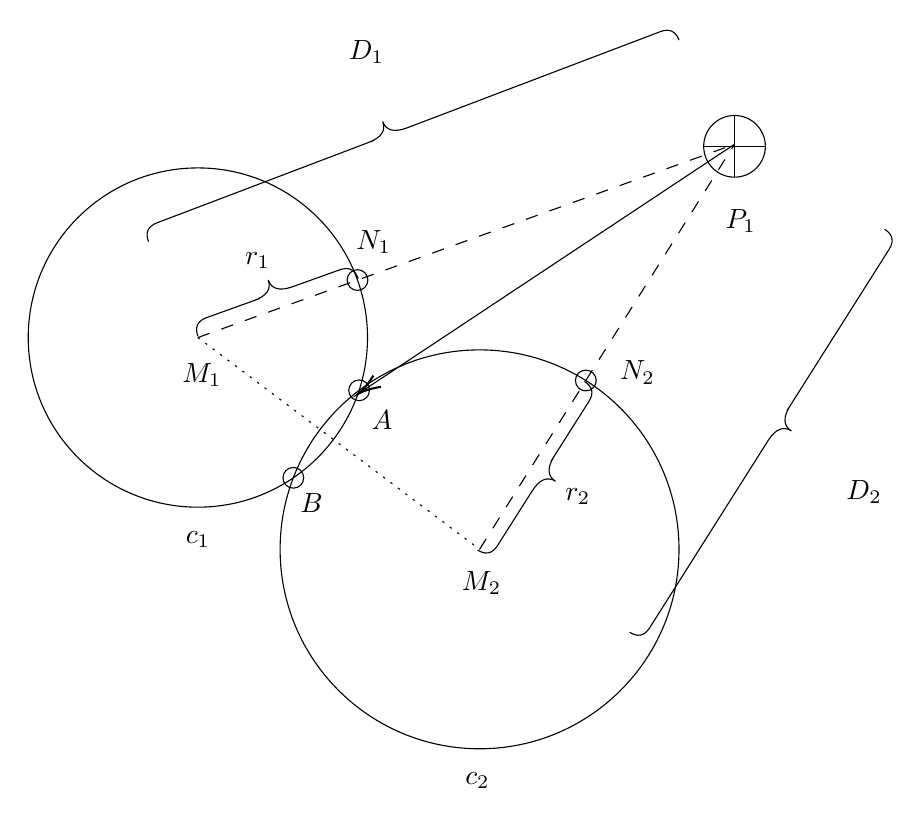
\begin{tikzpicture}[x=0.75pt,y=0.75pt,yscale=-1,xscale=1]
	%uncomment if require: \path (0,389); %set diagram left start at 0, and has height of 389

	%Shape: Circle [id:dp5885912263778241]
	\draw   (241.35,257.9) .. controls (241.35,204.83) and (284.38,161.81) .. (337.45,161.81) .. controls (390.52,161.81) and (433.54,204.83) .. (433.54,257.9) .. controls (433.54,310.97) and (390.52,354) .. (337.45,354) .. controls (284.38,354) and (241.35,310.97) .. (241.35,257.9) -- cycle ;
	%Shape: Ellipse [id:dp15448687207841338]
	\draw  [fill={rgb, 255:red, 255; green, 212; blue, 145 }  ,fill opacity=0 ] (120,155.87) .. controls (120,110.73) and (156.59,74.14) .. (201.73,74.14) .. controls (246.87,74.14) and (283.46,110.73) .. (283.46,155.87) .. controls (283.46,201) and (246.87,237.6) .. (201.73,237.6) .. controls (156.59,237.6) and (120,201) .. (120,155.87) -- cycle ;
	%Straight Lines [id:da6006500643796313]
	\draw  [dash pattern={on 0.84pt off 2.51pt}]  (201.73,155.87) -- (337.45,257.9) ;


	%Straight Lines [id:da5175683117647778]
	\draw  [dash pattern={on 4.5pt off 4.5pt}]  (201.73,155.87) -- (460.29,62.75) ;


	%Straight Lines [id:da33352637244621164]
	\draw  [dash pattern={on 4.5pt off 4.5pt}]  (337.45,257.9) -- (460.29,62.75) ;


	\draw   (445.43,63.74) .. controls (445.43,55.53) and (452.08,48.88) .. (460.29,48.88) .. controls (468.49,48.88) and (475.15,55.53) .. (475.15,63.74) .. controls (475.15,71.94) and (468.49,78.6) .. (460.29,78.6) .. controls (452.08,78.6) and (445.43,71.94) .. (445.43,63.74) -- cycle ; \draw   (445.43,63.74) -- (475.15,63.74) ; \draw   (460.29,48.88) -- (460.29,78.6) ;
	%Straight Lines [id:da19257704763660777]
	\draw    (460.29,62.75) -- (280.67,181.84) ;
	\draw [shift={(279,182.95)}, rotate = 326.45] [color={rgb, 255:red, 0; green, 0; blue, 0 }  ][line width=0.75]    (10.93,-3.29) .. controls (6.95,-1.4) and (3.31,-0.3) .. (0,0) .. controls (3.31,0.3) and (6.95,1.4) .. (10.93,3.29)   ;

	%Shape: Brace [id:dp007237602952800293]
	\draw   (279,127.47) .. controls (277.42,123.08) and (274.43,121.67) .. (270.04,123.25) -- (247.41,131.37) .. controls (241.14,133.62) and (237.21,132.55) .. (235.63,128.16) .. controls (237.21,132.55) and (234.86,135.88) .. (228.59,138.13)(231.41,137.12) -- (205.95,146.26) .. controls (201.56,147.83) and (200.15,150.82) .. (201.73,155.21) ;
	%Shape: Brace [id:dp7846975839966284]
	\draw   (336.46,258.23) .. controls (340.4,260.73) and (343.62,260.01) .. (346.12,256.07) -- (362.77,229.81) .. controls (366.34,224.18) and (370.09,222.62) .. (374.04,225.11) .. controls (370.09,222.62) and (369.91,218.55) .. (373.48,212.92)(371.87,215.45) -- (390.13,186.66) .. controls (392.63,182.72) and (391.91,179.5) .. (387.97,177) ;
	%Shape: Brace [id:dp41704229855363284]
	\draw   (433.54,12.55) .. controls (431.88,8.19) and (428.87,6.84) .. (424.51,8.5) -- (302.6,54.81) .. controls (296.37,57.18) and (292.42,56.18) .. (290.76,51.81) .. controls (292.42,56.18) and (290.13,59.54) .. (283.9,61.91)(286.71,60.84) -- (182.01,100.61) .. controls (177.65,102.27) and (176.3,105.28) .. (177.95,109.64) ;
	%Shape: Brace [id:dp09992687654682131]
	\draw   (409.76,297.86) .. controls (413.71,300.35) and (416.93,299.63) .. (419.42,295.69) -- (476.43,205.57) .. controls (480,199.94) and (483.75,198.37) .. (487.7,200.86) .. controls (483.75,198.37) and (483.56,194.3) .. (487.13,188.67)(485.52,191.2) -- (534.78,113.35) .. controls (537.27,109.41) and (536.55,106.19) .. (532.6,103.69) ;

	% Text Node
	\draw (203.71,174) node  [align=left] {$M_1$};
	% Text Node
	\draw (338.44,274.05) node  [align=left] {$M_2$};
	% Text Node
	\draw (230.48,118.73) node  [align=left] {$r_1$};
	% Text Node
	\draw (384.8,232.36) node  [align=left] {$r_2$};
	% Text Node
	\draw (201.78,253.22) node  [align=left] {$c_1$};
	% Text Node
	\draw (336.44,369.17) node  [align=left] {$c_2$};
	% Text Node
	\draw (463.26,99.73) node  [align=left] {$P_1$};
	% Text Node
	\draw (282.96,18.5) node  [align=left] {$D_1$};
	% Text Node
	\draw (522.7,230.5) node  [align=left] {$D_2$};
	% Text Node
	\draw (286.48,109.73) node  [align=left] {$N_1$};
	% Text Node
	\draw (413.48,172.73) node  [align=left] {$N_2$};
	% Text Node
	\draw (290.48,195.73) node  [align=left] {$A$};
	% Text Node
	\draw (256.48,235.73) node  [align=left] {$B$};

	\draw   (279.42, 181.3) circle [x radius= 5, y radius= 5]   ;
	\draw   (247.72, 223.44) circle [x radius= 5, y radius= 5]   ;
	\draw   (388.64, 176.57) circle [x radius= 5, y radius= 5]   ;
	\draw   (278.64, 128.17) circle [x radius= 5, y radius= 5]   ;
	\end{tikzpicture}
\caption{Körök metszete gömbfelületen}
\label{fig:spherical-sphere-intersection}
\end{figure}

\begin{tabular}{@{}ll@{}}
	\textbf{Jel} & \textbf{Leírás} \\
	$M_1$ & Előző pozíció \\
	$M_2$ & Következő pozíció \\
	$r_1$ & A jelenlegi időpont és $M_1$ időpontja között maximálisan megtehető út \\
	$r_2$ & A jelenlegi időpont és $M_2$ időpontja között maximálisan megtehető út \\
	$c_1$ & $M_1$ és $r_1$ által alkotott kör a gömbfelületen \\
	$c_2$ & $M_2$ és $r_2$ által alkotott kör a gömbfelületen \\
	$P_1$ & A felhasználó által kiválaszott célpozíció \\
	$D_1$ & A gömbfelületen vett távolság $P_1$ és $M_1$ között \\
	$D_2$ & A gömbfelületen vett távolság $P_1$ és $M_2$ között \\
	$N_1$ & A gömbfelület $M_1$ és $P_1$ pont által meghatározott \\
	& főkörén az a pont amely pontosan $r_1$ távolságra van $M_1$-től \\
	$N_2$ & A gömbfelület $M_2$ és $P_1$ pont által meghatározott \\
	& főkörén az a pont amely pontosan $r_2$ távolságra van $M_2$-től \\
	$A$ & $c_1$ és $c_2$ kör egyik metszéspontja \\
	$B$ & $c_1$ és $c_2$ kör másik metszéspontja \\
	& \\
\end{tabular}

Ebben az esetben a szereplő nem teljes sebességgel haladt a két pont között ezért ha félúton manipuláljuk, azt látjuk, hogy amellett, hogy mindkét ponthoz még eltudunk jutni, még van egy kis mozgásterünk ahol ugyanúgy eljutna a megadott időn belül $M_2$-be, képességeinek megfelelően. Meg kell határoznunk manipulálás közben, hogy $c_1$ és $c_2$ metszetében melyik pont van $P_1$ ponthoz a legközelebb.

Manipulálás kezdetekor válnak elérhetővé a kellő információk $c_1$ és $c_2$ adatainak a kiszámolásához. Ekkor számoljuk ki $A$ és $B$ pontot is. Ezt manipulálásonként csak egyszer számoljuk ki. Ekkor helyezzük el a két indikátor gömbcikket. A végén pedig el lesznek rejtve. Manipulálás közben pedig folyamatosan számljuk a legközelebbi pont függvényét.

\subsubsection{Két kör metszéspontjai gömbfelületen}

$M_1$ és $M_2$ világ pozíciók, és mivel a bolygó centruma a $(0, 0, 0)$ pontban helyetkedik el, ezért ezek egyben geocentrikus pontok is. A két kör metszéspontját gömbfelületen problémát átfogalmazhatjuk egy egyszerűbb problémává. Ha keresünk az $M_1$ és az origó által meghatározott vonalon egy pontot -- legyen $a$ -- és sugarat amivel egy akkora gömböt képez ami pontosan a $c_1$ körön metszi a bolygó gömbjét, és analóg módon $M_2$-höz egy $b$ pontot és sugarat. Akkor $a$ pont $c_1$ körrel és $b$ pont $c_2$ körrel egy-egy síkot határoznak meg, melyek metszésvonalán fog elhelyezkedni $A$ és $B$ pont is. Így a problémánk egy kör és egy egyenes metszetére redukálódott le.

\begin{figure}[h!]
	\centering

	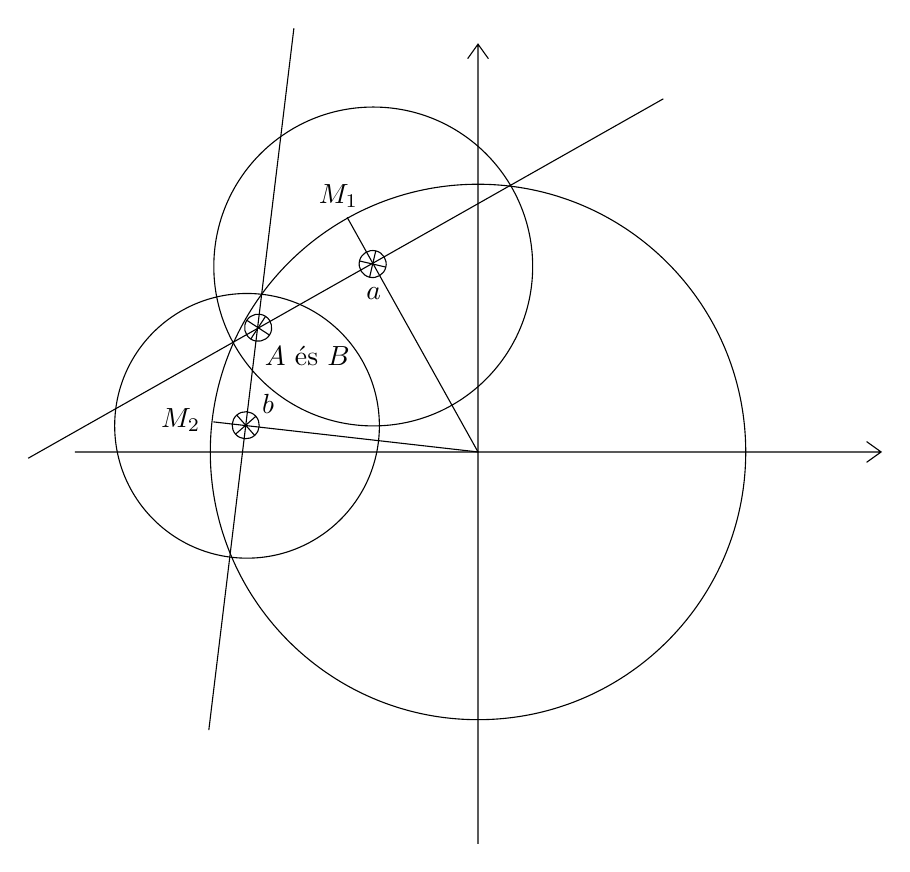
\begin{tikzpicture}[x=0.75pt,y=0.75pt,yscale=-1,xscale=1]
	%uncomment if require: \path (0,468); %set diagram left start at 0, and has height of 468

	%Shape: Circle [id:dp2263468573456704]
	\draw   (197.22,233.48) .. controls (197.22,162.24) and (254.97,104.49) .. (326.21,104.49) .. controls (397.44,104.49) and (455.19,162.24) .. (455.19,233.48) .. controls (455.19,304.72) and (397.44,362.47) .. (326.21,362.47) .. controls (254.97,362.47) and (197.22,304.72) .. (197.22,233.48) -- cycle ;
	%Shape: Circle [id:dp8130162816265305]
	\draw   (198.91,144.12) .. controls (198.91,101.69) and (233.3,67.3) .. (275.73,67.3) .. controls (318.15,67.3) and (352.54,101.69) .. (352.54,144.12) .. controls (352.54,186.54) and (318.15,220.93) .. (275.73,220.93) .. controls (233.3,220.93) and (198.91,186.54) .. (198.91,144.12) -- cycle ;
	%Shape: Circle [id:dp9863650593943492]
	\draw   (151.15,220.88) .. controls (151.15,185.67) and (179.7,157.12) .. (214.91,157.12) .. controls (250.13,157.12) and (278.68,185.67) .. (278.68,220.88) .. controls (278.68,256.1) and (250.13,284.65) .. (214.91,284.65) .. controls (179.7,284.65) and (151.15,256.1) .. (151.15,220.88) -- cycle ;
	%Straight Lines [id:da8253130424028727]
	\draw    (198.67,218.99) -- (326.21,233.48) ;


	%Straight Lines [id:da6219323829844645]
	\draw    (326.21,233.48) -- (263.16,120.43) ;


	%Shape: Axis 2D [id:dp7403279305833326]
	\draw  (132,233.48) -- (520.41,233.48)(326.21,37) -- (326.21,422.25) (513.41,228.48) -- (520.41,233.48) -- (513.41,238.48) (321.21,44) -- (326.21,37) -- (331.21,44)  ;
	\draw   (269.1,141.46) .. controls (269.92,137.95) and (273.43,135.77) .. (276.94,136.59) .. controls (280.44,137.41) and (282.62,140.92) .. (281.8,144.42) .. controls (280.98,147.93) and (277.48,150.11) .. (273.97,149.29) .. controls (270.46,148.47) and (268.28,144.96) .. (269.1,141.46) -- cycle ; \draw   (269.1,141.46) -- (281.8,144.42) ; \draw   (276.94,136.59) -- (273.97,149.29) ;
	\draw   (209.39,224.92) .. controls (207,222.22) and (207.26,218.1) .. (209.96,215.72) .. controls (212.66,213.34) and (216.78,213.59) .. (219.17,216.29) .. controls (221.55,218.99) and (221.29,223.12) .. (218.59,225.5) .. controls (215.89,227.88) and (211.77,227.62) .. (209.39,224.92) -- cycle ; \draw   (209.39,224.92) -- (219.17,216.29) ; \draw   (209.96,215.72) -- (218.59,225.5) ;
	%Straight Lines [id:da08394559625180209]
	\draw    (237.5,29.33) -- (196.5,367.5) ;


	%Straight Lines [id:da6409389593213928]
	\draw    (415.5,63.33) -- (109.5,236.5) ;


	\draw   (216.72,179.07) .. controls (213.7,177.11) and (212.85,173.06) .. (214.81,170.05) .. controls (216.78,167.03) and (220.82,166.18) .. (223.84,168.15) .. controls (226.86,170.11) and (227.71,174.15) .. (225.74,177.17) .. controls (223.77,180.19) and (219.73,181.04) .. (216.72,179.07) -- cycle ; \draw   (216.72,179.07) -- (223.84,168.15) ; \draw   (214.81,170.05) -- (225.74,177.17) ;

	% Text Node
	\draw (259,110.25) node  [align=left] {$M_1$};
	% Text Node
	\draw (183,218.25) node  [align=left] {$M_2$};
	% Text Node
	\draw (276,157.25) node  [align=left] {$a$};
	% Text Node
	\draw (225,210.25) node  [align=left] {$b$};
	% Text Node
	\draw (244,187.25) node  [align=left] {$A$ és $B$};


	\end{tikzpicture}





\caption{Átfogalmazott példa}
\label{fig:three-sphere-intersection}
\end{figure}



\begin{algorithm}[H]
	\caption{Két kör metszéspontjai gömbfelületen}
	\label{alg:intersection}
	\textbf{\underline{Function}} intersection($M_1, M_2, r_1, r_2, R$) ahol $R$ a bolygó sugara kilóméterben
	\begin{algorithmic}[1]
	\STATE $x_1 := M_1$ normalizálva \COMMENT{Valójában $M_1$ és $M_2$ vektor hossza már eleve 1}
	\STATE $x_2 := M_2$ normalizálva
	\STATE $rad_1 := r_1 / R$ \COMMENT{Átváltás radiánba}
	\STATE $rad_2 := r_2 / R$
	\STATE $q := x_1 \bullet x_2$ \COMMENT{A két vektor skaláris szorzata}
	\IF{$q^2 = 1$}
		\STATE return \COMMENT{A két kör nem metszheti egymást mert $M_1 = M_2$  vagy $M_1$ és $M_2$ a centrumhoz képest a szemközti oldalon állnak. Ebben az esetben vagy a körök minden pontja metszi egymást, vagy egy sem.}
	\ENDIF
	\STATE $a := \frac{cos(rad_1) - q \cdot cos(rad_2)}{1 - q^2}$
	\STATE $b := \frac{cos(rad_2) - q \cdot cos(rad_1)}{1 - q^2}$
	\STATE $x_0 := x_1 \cdot a + x_2 \cdot b$
	\IF{$x_0^2 > 1$}
		\STATE return \COMMENT{A két kör nem érintkezik.}
	\ENDIF
	\STATE $n := x_1 × x_2$
	\IF{$n^2 = 0$}
		\STATE return \COMMENT{A két kör középpontja vagy megegyezik vagy szemközt állnak.}
	\ENDIF
	\STATE $t := \sqrt{ \frac{1 - x_0 \bullet x_0}{n^2}}$
	\STATE $i_0 := x_0 + n \cdot t$
	\IF[Több eredmény csak pozitív $t$ esetén lehetséges]{$t > 0$}
		\STATE $i_1 := x_0 + n \cdot -t$
		\STATE return [$i_0$, $i_1$]
	\ELSE
		\STATE return [$i_0$]
	\ENDIF
	\end{algorithmic}
\end{algorithm}

\subsubsection{Körívek metszete gömbfelületen}

A legközelebbi pontok lehetnek $N_1$, $N_2$, $A$ és $B$. $N_1$ és $N_2$ viszont nem feltétlen helyezkednek el a metszés körívén. $N_1$ és $N_2$ akkor lesz érvényes, ha az adott $M$ és $P$ pont által meghatározott körív metszi az $A$ és $B$ által rajzolt körívet.

A \ref{fig:nearest-circle-intersection-examples}-es ábrán a $P_0$ szerű pontok megfelelnek mindkét kitételnek így további dolgunk nincs velük. A $P_1$ szerű pontok csak egy feltételnek felelnek meg. Az ő esetükben csak a másik kör középpontja felé kell interpolálnunk a szereplő pozícióját. A $P_2$ és $P_3$ pontok közötti különbség, hogy $P_2$-nél a legközelebbi pont maga a metszés mert se $N_1$ sem pedig $N_2$ nem a megfelelő köríven helyezkedik el.

\begin{figure}[h!]
	\centering
	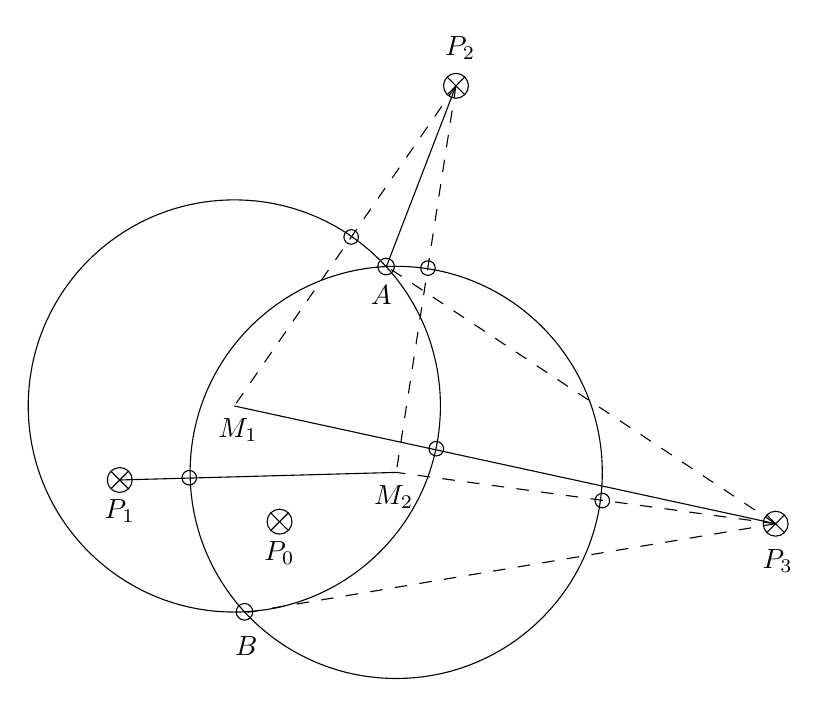
\begin{tikzpicture}[x=0.75pt,y=0.75pt,yscale=-1,xscale=1]
	%uncomment if require: \path (0,468); %set diagram left start at 0, and has height of 468

	%Shape: Circle [id:dp8166187689889921]
	\draw   (134.91,201.6) .. controls (134.91,146.76) and (179.37,102.3) .. (234.21,102.3) .. controls (289.05,102.3) and (333.5,146.76) .. (333.5,201.6) .. controls (333.5,256.43) and (289.05,300.89) .. (234.21,300.89) .. controls (179.37,300.89) and (134.91,256.43) .. (134.91,201.6) -- cycle ;
	%Shape: Circle [id:dp6909695032298264]
	\draw   (212.91,233.6) .. controls (212.91,178.76) and (257.37,134.3) .. (312.21,134.3) .. controls (367.05,134.3) and (411.5,178.76) .. (411.5,233.6) .. controls (411.5,288.43) and (367.05,332.89) .. (312.21,332.89) .. controls (257.37,332.89) and (212.91,288.43) .. (212.91,233.6) -- cycle ;
	%Flowchart: Summing Junction [id:dp009162364923596789]
	\draw   (250,257.33) .. controls (250,254.02) and (252.69,251.33) .. (256,251.33) .. controls (259.31,251.33) and (262,254.02) .. (262,257.33) .. controls (262,260.65) and (259.31,263.33) .. (256,263.33) .. controls (252.69,263.33) and (250,260.65) .. (250,257.33) -- cycle ; \draw   (251.76,253.09) -- (260.24,261.58) ; \draw   (260.24,253.09) -- (251.76,261.58) ;
	%Flowchart: Summing Junction [id:dp17652291932752062]
	\draw   (173,237.25) .. controls (173,233.94) and (175.69,231.25) .. (179,231.25) .. controls (182.31,231.25) and (185,233.94) .. (185,237.25) .. controls (185,240.56) and (182.31,243.25) .. (179,243.25) .. controls (175.69,243.25) and (173,240.56) .. (173,237.25) -- cycle ; \draw   (174.76,233.01) -- (183.24,241.49) ; \draw   (183.24,233.01) -- (174.76,241.49) ;
	%Flowchart: Summing Junction [id:dp4645172529660282]
	\draw   (489,258.33) .. controls (489,255.02) and (491.69,252.33) .. (495,252.33) .. controls (498.31,252.33) and (501,255.02) .. (501,258.33) .. controls (501,261.65) and (498.31,264.33) .. (495,264.33) .. controls (491.69,264.33) and (489,261.65) .. (489,258.33) -- cycle ; \draw   (490.76,254.09) -- (499.24,262.58) ; \draw   (499.24,254.09) -- (490.76,262.58) ;
	%Flowchart: Summing Junction [id:dp5476818076821499]
	\draw   (335,47.33) .. controls (335,44.02) and (337.69,41.33) .. (341,41.33) .. controls (344.31,41.33) and (347,44.02) .. (347,47.33) .. controls (347,50.65) and (344.31,53.33) .. (341,53.33) .. controls (337.69,53.33) and (335,50.65) .. (335,47.33) -- cycle ; \draw   (336.76,43.09) -- (345.24,51.58) ; \draw   (345.24,43.09) -- (336.76,51.58) ;
	%Straight Lines [id:da49460456729427316]
	\draw  [dash pattern={on 4.5pt off 4.5pt}]  (341,47.33) -- (234.21,201.6) ;


	%Straight Lines [id:da9864649930793872]
	\draw  [dash pattern={on 4.5pt off 4.5pt}]  (341,47.33) -- (312.21,233.6) ;


	%Straight Lines [id:da1538944910181792]
	\draw    (341,47.33) -- (307.5,134.33) ;


	%Flowchart: Connector [id:dp7527304205187331]
	\draw   (324,135.17) .. controls (324,133.23) and (325.57,131.67) .. (327.5,131.67) .. controls (329.43,131.67) and (331,133.23) .. (331,135.17) .. controls (331,137.1) and (329.43,138.67) .. (327.5,138.67) .. controls (325.57,138.67) and (324,137.1) .. (324,135.17) -- cycle ;
	%Flowchart: Connector [id:dp27712539160217364]
	\draw   (287,120.17) .. controls (287,118.23) and (288.57,116.67) .. (290.5,116.67) .. controls (292.43,116.67) and (294,118.23) .. (294,120.17) .. controls (294,122.1) and (292.43,123.67) .. (290.5,123.67) .. controls (288.57,123.67) and (287,122.1) .. (287,120.17) -- cycle ;
	%Straight Lines [id:da2513261195102452]
	\draw    (495,258.33) -- (234.21,201.6) ;


	%Flowchart: Connector [id:dp778704099897711]
	\draw   (328,222.17) .. controls (328,220.23) and (329.57,218.67) .. (331.5,218.67) .. controls (333.43,218.67) and (335,220.23) .. (335,222.17) .. controls (335,224.1) and (333.43,225.67) .. (331.5,225.67) .. controls (329.57,225.67) and (328,224.1) .. (328,222.17) -- cycle ;
	%Straight Lines [id:da16321655779119704]
	\draw  [dash pattern={on 4.5pt off 4.5pt}]  (495,258.33) -- (312.21,233.6) ;


	%Flowchart: Connector [id:dp00875038400506023]
	\draw   (408,247.17) .. controls (408,245.23) and (409.57,243.67) .. (411.5,243.67) .. controls (413.43,243.67) and (415,245.23) .. (415,247.17) .. controls (415,249.1) and (413.43,250.67) .. (411.5,250.67) .. controls (409.57,250.67) and (408,249.1) .. (408,247.17) -- cycle ;
	%Straight Lines [id:da46001771981700856]
	\draw  [dash pattern={on 4.5pt off 4.5pt}]  (495,258.33) -- (307.5,134.33) ;


	%Straight Lines [id:da4073168758118153]
	\draw  [dash pattern={on 4.5pt off 4.5pt}]  (495,258.33) -- (239,301.25) ;


	%Straight Lines [id:da30499884455793724]
	\draw    (179,237.25) -- (312.21,233.6) ;


	%Flowchart: Connector [id:dp8279616571890565]
	\draw   (209,236.17) .. controls (209,234.23) and (210.57,232.67) .. (212.5,232.67) .. controls (214.43,232.67) and (216,234.23) .. (216,236.17) .. controls (216,238.1) and (214.43,239.67) .. (212.5,239.67) .. controls (210.57,239.67) and (209,238.1) .. (209,236.17) -- cycle ;

	% Text Node
	\draw (305,148.33) node  [align=left] {$A$};
	% Text Node
	\draw (240,317.33) node  [align=left] {$B$};
	% Text Node
	\draw (236,213.33) node  [align=left] {$M_1$};
	% Text Node
	\draw (311,245.33) node  [align=left] {$M_2$};
	% Text Node
	\draw (343,29.33) node  [align=left] {$P_2$};
	% Text Node
	\draw (496,276.33) node  [align=left] {$P_3$};
	% Text Node
	\draw (256,272.33) node  [align=left] {$P_0$};
	% Text Node
	\draw (179,252.33) node  [align=left] {$P_1$};

	\draw   (307.33, 134.42) circle [x radius= 4, y radius= 4]   ;
	\draw   (239.09, 300.77) circle [x radius= 4, y radius= 4]   ;
	\end{tikzpicture}

\caption{Különböző esetek a legközelebbi pontok esetében}
\label{fig:nearest-circle-intersection-examples}
\end{figure}

\pagebreak

Először is meg kell határoznunk ezeket a metszéspontokat. Nevezzük $M_1$ és $P$ által meghatározott főkör és az $A$ és $B$ által meghatározott főkör metszetét $m_1$-nek. A hasonlóan $M_2$-höz tartozó metszetet pedig $m_2$-nek.

\begin{figure}[h!]
	\centering

	\begin{tikzpicture}[x=0.75pt,y=0.75pt,yscale=-1,xscale=1]
	%uncomment if require: \path (0,468); %set diagram left start at 0, and has height of 468

	%Shape: Circle [id:dp8166187689889921]
	\draw   (134.91,201.6) .. controls (134.91,146.76) and (179.37,102.3) .. (234.21,102.3) .. controls (289.05,102.3) and (333.5,146.76) .. (333.5,201.6) .. controls (333.5,256.43) and (289.05,300.89) .. (234.21,300.89) .. controls (179.37,300.89) and (134.91,256.43) .. (134.91,201.6) -- cycle ;
	%Shape: Circle [id:dp6909695032298264]
	\draw   (212.91,233.6) .. controls (212.91,178.76) and (257.37,134.3) .. (312.21,134.3) .. controls (367.05,134.3) and (411.5,178.76) .. (411.5,233.6) .. controls (411.5,288.43) and (367.05,332.89) .. (312.21,332.89) .. controls (257.37,332.89) and (212.91,288.43) .. (212.91,233.6) -- cycle ;
	%Flowchart: Summing Junction [id:dp5476818076821499]
	\draw   (248,27.5) .. controls (248,24.19) and (250.69,21.5) .. (254,21.5) .. controls (257.31,21.5) and (260,24.19) .. (260,27.5) .. controls (260,30.81) and (257.31,33.5) .. (254,33.5) .. controls (250.69,33.5) and (248,30.81) .. (248,27.5) -- cycle ; \draw   (249.76,23.26) -- (258.24,31.74) ; \draw   (258.24,23.26) -- (249.76,31.74) ;
	%Straight Lines [id:da49460456729427316]
	\draw  [dash pattern={on 4.5pt off 4.5pt}]  (254,27.5) -- (214,376.5) ;


	%Straight Lines [id:da9864649930793872]
	\draw    (254,27.5) -- (312.21,233.6) ;


	%Straight Lines [id:da1538944910181792]
	\draw  [dash pattern={on 4.5pt off 4.5pt}]  (254,27.5) -- (316,151.5) ;


	%Flowchart: Connector [id:dp7527304205187331]
	\draw   (281,138.17) .. controls (281,136.23) and (282.57,134.67) .. (284.5,134.67) .. controls (286.43,134.67) and (288,136.23) .. (288,138.17) .. controls (288,140.1) and (286.43,141.67) .. (284.5,141.67) .. controls (282.57,141.67) and (281,140.1) .. (281,138.17) -- cycle ;
	%Flowchart: Connector [id:dp27712539160217364]
	\draw   (242,102.17) .. controls (242,100.23) and (243.57,98.67) .. (245.5,98.67) .. controls (247.43,98.67) and (249,100.23) .. (249,102.17) .. controls (249,104.1) and (247.43,105.67) .. (245.5,105.67) .. controls (243.57,105.67) and (242,104.1) .. (242,102.17) -- cycle ;
	\draw  [dash pattern={on 0.84pt off 2.51pt}] (78.79,137.36) -- (467.29,298.6)(353.66,23.73) -- (192.42,412.23) ;
	%Flowchart: Connector [id:dp6649804334905414]
	\draw   (290,168.17) .. controls (290,166.23) and (291.57,164.67) .. (293.5,164.67) .. controls (295.43,164.67) and (297,166.23) .. (297,168.17) .. controls (297,170.1) and (295.43,171.67) .. (293.5,171.67) .. controls (291.57,171.67) and (290,170.1) .. (290,168.17) -- cycle ;
	%Flowchart: Connector [id:dp289603407901041]
	\draw   (213,354.17) .. controls (213,352.23) and (214.57,350.67) .. (216.5,350.67) .. controls (218.43,350.67) and (220,352.23) .. (220,354.17) .. controls (220,356.1) and (218.43,357.67) .. (216.5,357.67) .. controls (214.57,357.67) and (213,356.1) .. (213,354.17) -- cycle ;
	%Flowchart: Summing Junction [id:dp5805131421835337]
	\draw   (229.21,201.6) .. controls (229.21,198.83) and (231.45,196.6) .. (234.21,196.6) .. controls (236.97,196.6) and (239.21,198.83) .. (239.21,201.6) .. controls (239.21,204.36) and (236.97,206.6) .. (234.21,206.6) .. controls (231.45,206.6) and (229.21,204.36) .. (229.21,201.6) -- cycle ; \draw   (230.67,198.06) -- (237.74,205.13) ; \draw   (237.74,198.06) -- (230.67,205.13) ;
	%Flowchart: Summing Junction [id:dp23947035784845427]
	\draw   (307.21,233.6) .. controls (307.21,230.83) and (309.45,228.6) .. (312.21,228.6) .. controls (314.97,228.6) and (317.21,230.83) .. (317.21,233.6) .. controls (317.21,236.36) and (314.97,238.6) .. (312.21,238.6) .. controls (309.45,238.6) and (307.21,236.36) .. (307.21,233.6) -- cycle ; \draw   (308.67,230.06) -- (315.74,237.13) ; \draw   (315.74,230.06) -- (308.67,237.13) ;

	% Text Node
	\draw (305,148.33) node  [align=left] {$A$};
	% Text Node
	\draw (240,317.33) node  [align=left] {$B$};
	% Text Node
	\draw (236,213.33) node  [align=left] {$M_1$};
	% Text Node
	\draw (311,245.33) node  [align=left] {$M_2$};
	% Text Node
	\draw (254,14.33) node  [align=left] {$P_1$};
	% Text Node
	\draw (232,361.33) node  [align=left] {$m_1$};
	% Text Node
	\draw (312,171.33) node  [align=left] {$m_2$};

	\draw   (307.33, 134.42) circle [x radius= 4, y radius= 4]   ;
	\draw   (239.09, 300.77) circle [x radius= 4, y radius= 4]   ;
	\end{tikzpicture}

\caption{Körívek metszete gömbfelületen}
\label{fig:arc-intersection}
\end{figure}

\lstset{caption={Pontok által meghatározott körívek metszete}, label=src:arcIntersect}
\begin{lstlisting}[language={JavaScript}]
import { Vector3 } from 'three';

export function arcIntersection(p1: Vector3, pe1: Vector3, p2: Vector3, pe2: Vector3): Vector3 {
	const c1 = p1.clone().cross(pe1);
	const c2 = p2.clone().cross(pe2);
	const i1 = c1.clone().cross(c2);
	const i2 = c2.clone().cross(c1);
	const mid = p1.clone()
		.add(p2)
		.add(pe1)
		.add(pe2);
	return mid.dot(i1) > 0 ? i1 : i2;
}
\end{lstlisting}

Ha vesszük az $m_1, m_2, A$ és $B$ pontok és $P$ pont közti távolságot, akkor ezek alaján már meghatározhatjuk, hogy végül melyik pontot válasszuk.




















\lstset{caption={Legnagyobb még lehetséges bolygó sugár ahhoz, hogy az összes jelenlegi útja a szereplőknek még érvényes legyen.}, label=src:max-possible-radius}
\begin{lstlisting}[language={JavaScript}]
	public maxPossiblePlanetRadius$ = this.databaseService.currentLoreActors$.pipe(
		mergeMap(actors => of(...actors).pipe(mergeScan((acc, actor) =>
			of(...actor._states.nodes()).pipe(
				pairwise(),
				scan(
					(acc, [a, b]) => {
						if (a.value.maxSpeed !== undefined) {
							acc.lastMaxSpeed = a.value.maxSpeed; // km/h
						}
						this._va.copy(a.value.position as Vector3);
						this._vb.copy(b.value.position as Vector3);
						const time = Math.abs(b.key.unix - a.key.unix); // s
						const maxDistance = acc.lastMaxSpeed * (time / 3600);
						const angle = this._va.angleTo(this._vb);
						const maxRadius = maxDistance / angle;
						if (acc.maxRadius >= maxRadius) {
							acc.maxRadius = maxRadius;
						}
						return acc;
					},
					{
						lastMaxSpeed: Actor.DEFAULT_MAX_SPEED,
						maxRadius: Infinity
					}
				),
				map(({ maxRadius }) => (acc > maxRadius ? maxRadius : acc))
			), Infinity))),
		shareReplay(1)
	);

\end{lstlisting}






























\subsection{Technológiák}

\begin{table}[H]
	\centering
	\begin{tabular}{ | m{0.20\textwidth} | m{0.80\textwidth} | }
		\hline
		\textbf{Csomag} & \textbf{Szerep} \\
		\hline \hline
		\emph{Angular} \cite{Angular} & A fő keretrendszer, biztosítja a build eszközöket mint Webpack. \\
		\hline
		\emph{RxDB} \cite{RxDB} & Reaktív interfészt biztosít a böngészők IndexedDB adatbázisaihoz. \\
		\hline
		\emph{NgRx} \cite{NgRx} & Reaktív állapot menedzsment. \\
		\hline
		\emph{Three.js} \cite{Three} & WebGL könyvtár a 3D grafikai elemekhez. \\
		\hline
		\emph{Tween.js} \cite{Tween} & Interpolációs könyvtár. \\
		\hline
		\emph{FontAwesome} \cite{FontAwesome} & Ikon könyvtár.  \\
		\hline
		\emph{TypeScript} \cite{TypeScript} & Típusos JavaScript kiegészítő.  \\
		\hline

		\emph{Sass} \cite{Sass} & CSS kiegészítő könyvtár.  \\
		\hline
	\end{tabular}
	\caption{Az alkalmazás technológiái}
	\label{tab:technologies}
\end{table}

\begin{table}[H]
	\centering
	\begin{tabular}{ | m{0.20\textwidth} | m{0.80\textwidth} | }
		\hline
		\textbf{Eszköz} & \textbf{Szerep} \\
		\hline \hline
		\emph{NPM} \cite{NPM} & JavaScript csomagkezelő eszköz.  \\
		\hline
		\emph{GitHub} \cite{Github} & Online git repository.  \\
		\hline
		\emph{Travis-CI} \cite{Travis} & Online build és deployment.  \\
		\hline
	\end{tabular}
	\caption{Devops eszközök}
	\label{tab:technologies}
\end{table}
